\chapter{Introduction}
\label{ch:Introduction}

\stress{\textbf{Disclaimer to this document:} 
This is a template with some additional thesis information and a sample structure. 
The structure includes the chapters most commonly needed in a thesis. 
Neither the order nor the chapter titles are fixed and will most likely 
have to be adapted to your specific thesis. 
However, the notes here should help you to get an idea what each chapter 
could be about and how to use this template. 
When in doubt, please talk to your supervisor(s).}

Your thesis should start with an introduction. The introduction is supposed to motivate your thesis.
Discuss the relevance of your topic, why are you looking into it, why is it relevant in the field? Cite important research related to your motivation.
Briefly state the problem as in the abstract and repeat the contribution, for example in the form of research questions. 

Give an outline of your thesis.

Testing the glossaries package \gls{rmse}


Below, you will find an example figure (\Cref{fig:example}). Please use the caption of your figures to describe everything in the figure, additionally to what you have written about the figure in the text. Everyone should be able to understand the figure just reading its caption.

\begin{figure}[h!]%
\centering
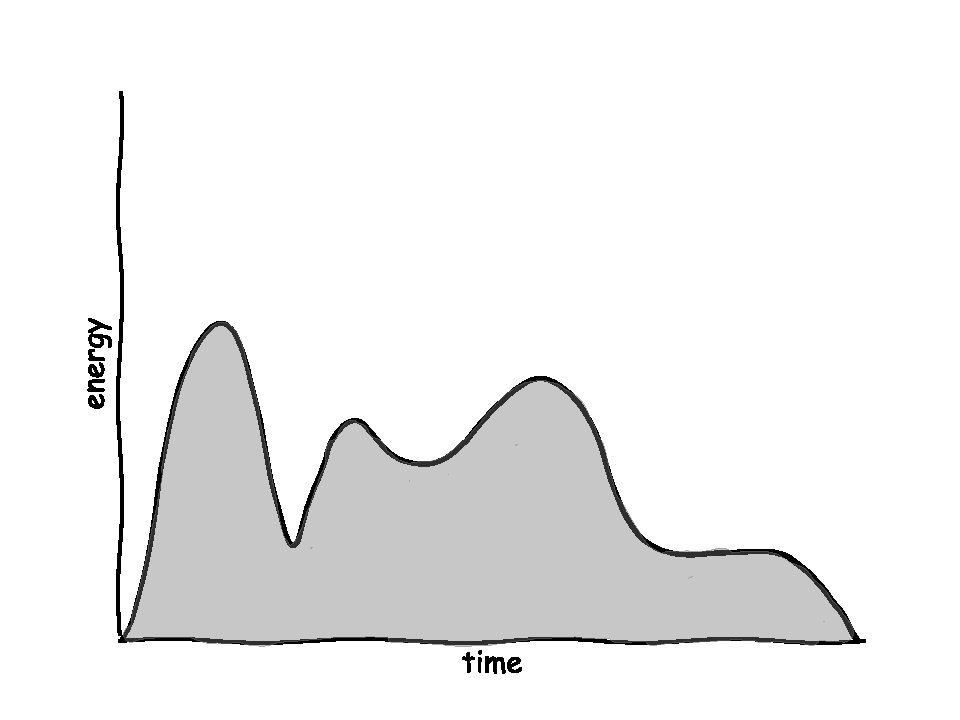
\includegraphics[width=0.5\columnwidth]{plots/Figure_2_demand}%
\caption{This is an example figure. It shows a fictional demand of energy (in grey) over time.}%
\label{fig:example}%
\end{figure}

\section{The GEFCom2014 Dataset}
\label{sec:gefcom-dataset}

In order to compare different energy forecasting methods, 
\Textcite{Hong2016} organized the Global Energy Forecasting Competition 2014 (GEFCom2014), 
a probabilistic energy forecasting competition with four tracks: 
electric load, electric price, wind power and solar power forecasting. 
The competition attracted 581 participants from 61 countries. 

The Global Energy Forecasting Competition took place the first time in 2012. 
In the 2014 competition, they upgraded the competition with three features: 
\begin{enumerate}
    \item instead of point forecasts, probabilistic forecasts were used;
    \item four forecasting tracks were used: electric load (L track), 
    electric price (P track), wind power (W track) and solar power (S track);
    \item incremental data releases on a weekly basis to mimic real world forecasting.
\end{enumerate}

In this thesis, we will only look at the solar power track. 
In this track, the task is to predict the power generation of three 
solar power plants (the so called zones) in Australia. 
The prediction is on a rolling basis for \(\SI{24}{\hour}\) ahead. 
The forecasts are to be issued at midnight each day for the next \(24\) hours. 
\(15\) tasks are provided for the challenge. In each one, the participants need to 
provide one month of forecasts, so \(28\)-\(31\) days.
For the forecasts, different prediction variables from the 
European Centre for Medium-Range Weather Forecasts (ECMWF) are provided. 
They are shown in Table \ref{table:predictors}.
Power measurements are also provided, but only over the training period. 

In order to become familiar with the data, only the last twelve of the 15 available tasks 
from April 2013 to June 2014 counted towards the final score.
The final score was calculated using a linear increasing weighted mean over the scores from the different tasks: 
The first task got weight \(1/78\), the second \(2/78\), etc. 
in order to promote models that improve over time. The division by \(78\) is so that the 
weights sum to \(1\).
Since we will evaluate the models on the dataset as a whole instead of on a monthly different basis, 
we will take the mean over the \(12\) different losses.

\begin{table}[ht]
\caption[Predictors for the GEFCom2014-S track]{Predictors for the GEFCom2014-S track \par Adapted from Table 10 in \cite{Hong2016}}
\label{table:predictors}
\rowcolors{2}{white}{gray!25}
\footnotesize
\begin{tabularx}{\textwidth}{llX}
    \toprule
    \tableheads Variable name & \tableheads Units & \tableheads Comments \\
    \midrule
    Total column liquid water (tclw) & \(\si{\kilo\gram\per\square\metre}\) & Vertical integral of cloud liquid water content \\
    Total column ice water (tciw) & \(\si{\kilo\gram\per\square\metre}\) & Vertical integral of cloud ice water content \\
    Surface pressure (SP) & \(\si{\pascal}\) & \\
    Relative humidity at \(\SI{1000}{\milli\barsi}\) (r) & \(\%\) & Relative humidity is defined with respect to saturation of
                                                                  the mixed phase, i.e., with respect to saturation over ice
                                                                  below \(\SI{-23}{\degreeCelsius}\) and with respect to saturation over water 
                                                                  above \(\SI{0}{\degreeCelsius}\). In the regime in between, a quadratic
                                                                  interpolation is applied. \\
    Total cloud cover (TCC) & \(0\)-\(1\) & TCC derived from model levels using the
                                            model's overlap assumption \\
    \(10\)-metre \(U\) wind component (\(10u\)) & \(\si{\metre\per\second}\) & \\
    \(10\)-metre \(V\) wind component (\(10v\)) & \(\si{\metre\per\second}\) & \\
    \(2\)-metre temperature (\(2T\)) & \(\si{\kelvin}\) & \\
    Surface solar rad down (SSRD) & \(\si{\joule\per\square\metre}\) & Accumulated field \\
    Surface thermal rad down (STRD) & \(\si{\joule\per\square\metre}\) & Accumulated field \\
    Top net solar rad (TSR) & \(\si{\joule\per\square\metre}\) & Net solar radiation at the top of the atmosphere. Accumulated field \\
    Total precipitation (TP) & \(\si{\metre}\) & Convective precipitation \(+\) stratiform precipitation (CP + LSP). Accumulated field \\
    \bottomrule
\end{tabularx}
\end{table}

\section{Spline Quantile Function RNNs}
\label{sec:sqf-rnn}

\Textcite{Gasthaus2019} proposed a method for probabilistic forecasting by modeling 
the quantile function with monotonic regression splines. 
The proposed \gls{sqfrnn} model combines the ability to forecast time series 
from recurrent neural networks which was already done by the DeepAR model from \Textcite{Salinas2017}
with the flexibility of being able to 
model the quantile functions with linear splines. 

Let \(x_1, \ldots, x_n \in \R^D\) be the predictor values and 
\(z_1, \ldots, z_n \in \R\) be the target time series. Also, let \(\Theta\) 
be the model parameters, \(\boldsymbol{h}_t\) the network output of 
time step \(t\) and \(\theta_t\) the parameters of the conditional distribution \(\P(z_t | \theta_t)\).
The model works as follows:
Compute the network output \(\boldsymbol{h}_t = h(\boldsymbol{h}_{t-1}, z_{t-1}, x_t, \Theta)\) 
as well as the parameters \(\theta_t = \theta(\boldsymbol{h}_t, \Theta)\) for the distribution
\(\P(z_t | \theta_t)\). \(h(\cdot)\) is a multi-layer RNN with 
LSTM cells and \(\theta(\cdot)\) is a projection layer. 
The quantiles are then used to calculate the loss and train the model parameters \(\Theta\).
The process is illustrated in Figure \ref{fig:deepar-training}.

\begin{figure}[h]%
    \centering
    \begin{tikzpicture}[yscale=-1,node distance=-\pgflinewidth]
    \tikzset{ReceptorNode/.style={circle, draw=black, fill=lightblue, thick, inner sep=2pt, minimum size=30pt}}
    \tikzset{Placeholder/.style={circle, thick, inner sep=2pt, minimum size=30pt}}
    \tikzset{Connection/.style={->, line width=0.5mm}}
    \newcommand{\mynode}[3]{
        \node[ReceptorNode] (circ-#2) at (#1, 0) {\(\boldsymbol{h}_{#2}\)};
        \node (x-#2) at (#1, 1.5) {\(x_{#2}, y_{#3}\)};
        \node (y-#2) at (#1, -1.5) {\(\P(y_{#2}|\boldsymbol{h}_{#2})\)};

        \draw[Connection] (circ-#2) -- (y-#2);
        \draw[Connection] (x-#2)    -- (circ-#2);
    }
    \newcommand{\placeholder}[2]{
        \node[Placeholder] (circ-#2) at (#1, 0) {\(\cdots\)};
        \node (x-#2) at (#1, 1.5) {};
        \node (y-#2) at (#1, -1.5) {\phantom{\(\P(y_{#2}|\boldsymbol{h}_{#2})\)}};
    }
    \newcommand{\connect}[2]{
        \draw[Connection] (circ-#1) -- (circ-#2);
    }

    % Create nodes
    \mynode{1 * 2.5}{1}{0}
    \onslide<2->{
        \mynode{2 * 2.5}{2}{1}
        \connect{1}{2}    
    }
    \onslide<2->{
        \mynode{3 * 2.5}{3}{2}
        \connect{2}{3}    
    }
    \onslide<3->{
        \placeholder{4 * 2.5}{4}
        \connect{3}{4}
    }
    % Last node is called "n"
    \onslide<4->{
        \mynode{5*2.5}{n}{n-1}
        \connect{4}{n}
    }
\end{tikzpicture}
    \caption{DeepAR Training}%
    \label{fig:deepar-training}%
\end{figure}

For the prediction step, the target time series are not known. 
The known history of the time series \(z_1, \ldots, z_{t_0}\) is fed into the 
model and for \(t > t_0\), samples \(\tilde{z}_t \sim \P(z_t | \theta_t)\) 
are generated and fed back into the model for the next time step.
The process is illustrated in Figure \ref{fig:deepar-predicting}.

\begin{figure}[h]%
    \centering
    \begin{tikzpicture}[yscale=-1,node distance=-\pgflinewidth]
    \tikzset{ReceptorNode/.style={circle, draw=black, fill=lightblue, thick, inner sep=2pt, minimum size=30pt}}
    \tikzset{Placeholder/.style={circle, thick, inner sep=2pt, minimum size=30pt}}
    \tikzset{Connection/.style={->, line width=0.5mm}}
    \newcommand{\mynode}[3]{
        \node[ReceptorNode] (circ-#2) at (#1, 0) {\(\boldsymbol{h}_{#2}\)};
        \node (x-#2) at (#1, 1.5) {\(x_{#2}, z_{#3}\)};
        \node (y-#2) at (#1, -1.5) {\(\P(z_{#2}|\boldsymbol{h}_{#2})\)};

        \draw[Connection] (circ-#2) -- (y-#2);
        \draw[Connection] (x-#2)    -- (circ-#2);
    }
    \newcommand{\mynodewithresult}[3]{
        \node[ReceptorNode] (circ-#2) at (#1, 0) {\(\boldsymbol{h}_{#2}\)};
        \node (x-#2) at (#1, 1.5) {\(x_{#2}, z_{#3}\)};
        \node (y-#2) at (#1, -1.5) {\(\P(z_{#2}|\boldsymbol{h}_{#2})\)};
        \node (z-#2) at (#1, -2.5) {\(\tilde{z}_{#2}\)};

        \draw[Connection] (circ-#2) -- (y-#2);
        \draw[Connection] (x-#2)    -- (circ-#2);
        \draw[Connection] (y-#2)    -- (z-#2);
    }
    \newcommand{\mynodewithresultinputsampled}[3]{
        \node[ReceptorNode] (circ-#2) at (#1, 0) {\(\boldsymbol{h}_{#2}\)};
        \node (x-#2) at (#1, 1.5) {\(x_{#2}, \tilde{z}_{#3}\)};
        \node (y-#2) at (#1, -1.5) {\(\P(z_{#2}|\boldsymbol{h}_{#2})\)};
        \node (z-#2) at (#1, -2.5) {\(\tilde{z}_{#2}\)};

        \draw[Connection] (circ-#2) -- (y-#2);
        \draw[Connection] (x-#2)    -- (circ-#2);
        \draw[Connection] (y-#2)    -- (z-#2);
    }
    \newcommand{\placeholder}[2]{
        \node[Placeholder] (circ-#2) at (#1, 0) {\(\cdots\)};
        \node (x-#2) at (#1, 1.5) {};
        \node[opacity=0] (y-#2) at (#1, -1.5) {\(\P(z_{#2}|h_{#2})\)};
    }
    \newcommand{\connect}[2]{
        \draw[Connection] (y-#1)    -- (circ-#2);
        \draw[Connection] (circ-#1) -- (circ-#2);
    }

    % Create nodes
    \mynode{1 * 2.5}{T}{T-1}
    \draw[Connection] ([xshift=-0.5cm]circ-T.west) -- (circ-T);
    \onslide<2->{
        \mynodewithresult{2 * 2.5}{T+1}{T}
        \connect{T}{T+1}
    }
    \onslide<3->{
        \mynodewithresultinputsampled{3 * 2.5}{T+2}{T+1}
        \connect{T+1}{T+2}
    }
    \onslide<4->{
        \placeholder{4 * 2.5}{T+3}
        \connect{T+2}{T+3}
    }
    % Last node is called "T+n"
    \onslide<5->{
        \mynodewithresultinputsampled{5*2.5}{T+n}{T+n-1}
        \connect{T+3}{T+n}
    }
\end{tikzpicture}
    \caption{DeepAR Predicting}%
    \label{fig:deepar-predicting}%
\end{figure}

While the DeepAR model is trained by maximizing the likelihood function, 
the SQF-RNN model is trained by minimizing the CRPS (see \ref{ch:crps}) 
which can be computed effectively for spline-based quantile functions.

A linear spline with \(L\) pieces is of the form 
\[ s(x; \gamma, b, d) = \gamma + \sum_{l=0}^L b_l (x - d_l)_+, 
\quad b, d \in \R^{L+1}. \]
Since we want a monotone spline, we need to create constraints for \(b_l\) and \(d_l\).
We want \(d_l < d_{l+1}\) for ordered knot positions. To achieve this 
in the neural network, we set \(d_0 = 0\) and \(d_l = \sum_{j=1}^l \delta_j\), 
where \(\delta_j \geq 0\) and \(\sum_{j=1}^L \delta_j = 1\) since the domain 
of the quantile function is \([0, 1]\). 
We also want monotonicity: the slope \(m_l\) between two knots is given by 
\(m_l = \sum_{j=0}^l b_j\). We need to make sure that \(m_l \geq 0 \forall l\).
If we set \(b_l = \beta_l - \beta_{l-1}\) and \(b_0 = \beta_0\) with \(\beta_l \geq 0 \forall l\), 
we get \(m_l = \sum_{j=0}^l b_j = \beta_l \geq 0\).
We can therefore model our spline with the parameter 
\(\theta = (\gamma, \beta, \delta)\), \(\gamma \in \R, \beta \in [0,\infty)^{L}, 
\delta \in \set{ \delta \in [0,1]^L: \sum_{j=1}^L \delta_j = 1 }\).

\section{Nearest Neighbor Quantile Filters}
\label{sec:nnqf}

\Textcite{Ordiano2019} proposed a method for probabilistic 
energy forecasting using quantile regression based on a \gls{nnqf}. 
The method works as follows: first, the training set is modified 
by using the Nearest Neigbor Quantile Filters so that 
the training data directly represents a probabilistic distribution. 
Then, a regression model like an artificial neural network can 
train on this modified data set and learn the quantile function.

The preprocessing of the NNQF method includes multiple steps. 
Firstly, we search the \(k\) nearest neighbors 
for every \(x_i\).
The distance metric can be any distance metric on \(\R^D\), 
the euclidean metric is used often.
Let \(J \subset \set{1, \ldots, n}\) be the indices of 
those nearest neighbors. 
The probabilistic distribution of \(y_i\) can be approximated 
by calculating the empirical quantile \(\tilde{y}_{(q),i}\) of 
\(\set{y_j \;|\; j\in J}\) for each \(q \in \set{0.01, \ldots, 0.99}\). 

After repeating this procedure for each entry in the time series, 
we get vectors 
\[ \tilde{y}_{(q)} = \begin{pmatrix}
    \tilde{y}_{(q), 1} \\ 
    \vdots \\
    \tilde{y}_{(q), n}
\end{pmatrix} \]
that form the modified training set combined with the 
predictors \(X = (x_1, \ldots, x_n)\).

Because we work with a time series, adjacent points are correlated. 
That's the reason why we use lag features: 
instead of only \(x_i\), we are using \(x_i, \ldots, x_{i-H+1}\) to 
predict the target data. \(H\) is called lag size.

With the modified training set, one can now train the regression model 
for each quantile and fit the function 
\[ f_\theta(x_i, \ldots, x_{i-H+1}) = \tilde{y}_{(q), i}. \]
Common examples are polynomial regression or 
artificial neural networks. 

This method has three main advantages: 
\begin{enumerate}
    \item The technique for the quantile regression is not specified, 
    any technique can be used,
    \item the calculation of the nearest neighbors and the modified 
    training set only needs to be done once, you can save time when 
    using multiple quantile regressions. 
    \item The original dataset does not need to be saved afterwards, 
    we only need the weights of the regression model for predicting.
\end{enumerate}

In comparison to most other \(k\)-Nearest Neighbors quantile 
regression techniques, the nearest neighbors are only calculated once 
and then the regression model is trained on the modified training data. 
A regular \(k\)-Nearest Neighbor quantile regression algorithm 
calculates the nearest neighbors every time when a forecast is conducted 
(cf. \Textcite{Ma2015}, p. 3 ff) which is computationally more expensive in the long run.